\documentclass[SE,authoryear,toc]{lsstdoc}
%\documentclass{article}

% lsstdoc documentation: https://lsst-texmf.lsst.io/lsstdoc.html
\input{meta}

% Package imports go here.
\usepackage{graphicx}
% Local commands go here.

%If you want glossaries
%\input{aglossary.tex}
%\makeglossaries

\title{SIT-COM Work Management and Organization}

% Optional subtitle
% \setDocSubtitle{A subtitle}

\author{%
Sandrine Thomas, Leanne Guy, Austin Roberts
}

\setDocRef{SITCOMTN-023}
\setDocUpstreamLocation{\url{https://github.com/lsst-sitcom/sitcomtn-023}}
\date{\vcsDate}

% Optional: name of the document's curator
% \setDocCurator{The Curator of this Document}

\setDocAbstract{This management plan covers the activity coordination structure of the System Integration Test and Commissioning (SIT-COM) team. }

% Change history defined here.
% Order: oldest first.
% Fields: VERSION, DATE, DESCRIPTION, OWNER NAME.
% See LPM-51 for version number policy.
\setDocChangeRecord{%
  \addtohist{1}{YYYY-MM-DD}{Unreleased.}{Leanne Guy}
  \addtohist{2}{2022-05-12}{Unreleased.}{Sandrine Thomas}
  \addtohist{3}{2022-06-01}{Added section on linkages. Minor clarifications and formatting.}{Patrick Ingraham}
}
%


\begin{document}

% Create the title page.
\maketitle
% Frequently for a technote we do not want a title page  uncomment this to remove the title page and changelog.
% use \mkshorttitle to remove the extra pages

% ADD CONTENT HERE
% You can also use the \input command to include several content files.
\section{Introduction}
The goal of this document is to define the process for an efficient and timely organization of the work required for the successful commissioning of the Vera C. Rubin Observatory. 
This process includes defining the current SIT-Com priorities along with their coordination both at the SIT-Com and Project level. 
The global prioritization of activities is defined by three primary use-cases: (i) the level 2 and level 3 milestones described in P6, (ii) planned work not linked to a milestone (including the managerial work from the SIT-Com leadership team (SCLT)), and (iii) unplanned emergent issues.

This document first lays down the different use cases along with their appropriate processes and the prioritization strategy.
From these uses cases, we defined the requirements for a Jira-based workflow that will satisfy our needs, including ticket status, ticket types, the review process, and a dashboard. 
Finally, we describe how this Jira project interfaces with the other existing projects. 

\section{Work Management Needs}
\subsection{Processes}
As mentioned in the introduction, there are three main use cases for the work management process. 
\subsubsection{Milestone Tracking}
\label{sec:milestone_tracking}
The P6 tool holds the integration master schedule for the Rubin project where two sets of milestones are defined for SIT-Com: Level 2 (L2) and Level 3 (L3). 
Each L2 and L3 milestone is achieved when the list of associated stories, which are generally grouped into Epics, are completed.
This is further discussed in section \ref{sec:jira}.
Both L2 and L3 milestones are to be reported on weekly at the SIT-Com leadership meetings, especially if delays/blockers are encountered, in which case the impact on the schedule/cost/performance may need to be elevated to the project management level.

\subsubsection{Planned Activities not linked to a milestone}
The workflow, tickets types and review processes are similar to the milestone tracking use case, except that the work itself is not tied to a milestone, and therefore not tracked at the project level.
Planned activities not linked to a milestone can be grouped into epics and/or individual stories, depending on the nature of the task.


\subsubsection{Emergent Tasks}
Finally, the emergent tasks use case is a mechanism for anyone on the commissioning team to enter unforeseen issues and bugs encountered during commissioning activities. 
They do not need to be linked to an epic or a milestone when being created. 
The triage will be done by the SCLT to verify and/or define assignees as well as priorities relative to other work. 
During this process they will either be added to an active epic or put on the backlog for later scheduling.

\subsection{Prioritization strategy}
Activities are assigned a priority level to help guide their order of implementation.
The priority level is first assigned by the reporter of the ticket and then discussed and updated by the SCLT if it is appropriate to do so.
The 5 priority levels are defined as follows:
\begin{itemize}
\item{\bf Critical}: when a ticket is flagged as critical, the assignee(s) are expected to focus only on this particular activity. 
As a result, each person should have only one critical activity to work on at a given time and managers should adjust the schedule to allow for the other activities to wait, including meetings. 
Usually, the associated ticket (most likely bugs) are blocking critical path activities that are ON-GOING if not done or will result in a severe hampering of night-time operations. 
%This should hardly ever happen and should only last for a short period of time (of the order of a few days). 

\item{\bf High} - A ticket is flagged as high priority when the activity is needed to be completed in short order (within a couple of weeks) and at risk of hitting the critical path if not worked on immediately and with a high amount of dedicated time. 
Essentially, a single person should only EVER have one of these at a time, potentially combined with other tasks with lower criticality. 

\item{\bf Medium (default)} - This is the default level and most tasks will be flagged as such. 
They correspond to off critical path items that have some wiggle room on deadline. 
Task should be mapped to a milestone, a planned activity or a roadmap (in the case of broader teams).  
Each person should have no more than ~3 of these.

\item{\bf Low} A ticket is flagged as low when it is a nice-to-have not immediately needed. 
They receive attention when someone has time and  should be worked on a MINIMUM of a few hours per week. 
They can be elevated in criticality if need be at a later date by the coordinator of the ticket.  

\item{\bf Undefined} These are the backlogged tickets that no one should be working on.
\end{itemize}

It is important that the SIT-Com managers and coordinators regularly check the priorities against the overarching project schedule as well as the list of tasks per person to ensure people are not overbooked. 


\section{The SIT-Com Work Management Jira Project}
\label{sec:jira}
Based on the use-cases discussed in the previously, this section describes the different resulting configurations for the Jira project. 

There are 5 different ticket types within this Jira project.
There are two levels of milestones called L2 and L3, linked to the P6 schedule, as described in section \ref{sec:milestone_tracking}.
Each of the {\bf L2 milestones} requires its associated number of {\bf L3 milestones} to be accomplished before being reviewed. 
Each L3 milestone is further decomposed into {\bf Epics} and tracked by one of the SCLT coordinators. 

The epics gather {\bf stories}, themselves relating to {\bf tasks}. 
The stories and tasks are respectively defined by a SIT-Com member and anyone on the project. 
pics, stories and tasks can be defined independently of a milestone when appropriate.

\subsection{Ticket Types}
The fields required for the different tickets include the title, summary, description, component, assignee, priority. 
The other fields are Start Date (Non milestones), End Date (non milestones), Labels, Reviewers, Approved by.  
The fields specific to each ticket type is listed below.
\begin{itemize}
\item{Milestones}: Milestone level (required), Success Criteria, Due Date, L2 Milestone, L3 Milestones, included Epics
\item{Epics}: Epic name, Sprint, Story points, Supported Milestones, Included Stories/Bugs
\item{Story/Bug}: Epic Link, Sprint, Story Points, Supported Epic, Related Issues, Needs to be done before/after
\item{Tasks}: Story Points, Needs to be done before/after
\end{itemize}

\subsubsection{Linkages}
The Rubin project contains numerous Jira projects.
Generally, a Jira project is associated with a team (e.g. DM) and/or a specific purpose (e.g. risk management).
The projects that will often contain information pertinent to SIT-Com personnel are described in section \ref{sec:other_jiras}.

Jira provides a large array of link types between the different ticket types, many of which are ambiguous in their meaning. 
This section describes which link types are available to which ticket type, and how the SIT-Com team defines their significance.

\begin{enumerate}
  \item \textbf{Common to all ticket types}
  \begin{itemize}
    \item \emph{blocks}: Prevents the linked ticket from being actionable.
    \item \emph{is blocked by}: The affected ticket of \emph{blocks}.
    \item \emph{relates to}: A non-binding relationship that exists to point users to historical or possibly pertinent information.
  \end{itemize}

  \item \textbf{Milestones:}
  \begin{itemize}
    \item \emph{contains}: Links an epic that must be accomplished to complete the milestone.
  \end{itemize}

  \item \textbf{Epics:}
  \begin{itemize}
    \item \emph{is contained by}: Links the associated milestone. 
    This is the affected ticket of \emph{contains}.
  \end{itemize}

  \item \textbf{Stories, Tasks, and Bugs:}
  \begin{itemize}
    \item \emph{clones}: Current ticket has been copied from this linked ticket. 
    It provides the basis of the ticket but may not have identical content.
    \item \emph{is cloned by:} The affected ticket of \emph{clones}.
  \end{itemize}
\end{enumerate}



\subsection{Workflows}
There will be two different workflows, depending on whether the ticket type is a milestone or not, as shown in Figure \ref{fig:workflow}. 
The main differences are the acknowledged and invalid states available in the non-milestone case.  
This comes from the nature of the milestones ticket being only an achieved goal instead of an activity that needs to be done. 

\begin{figure}[h]
\begin{center}
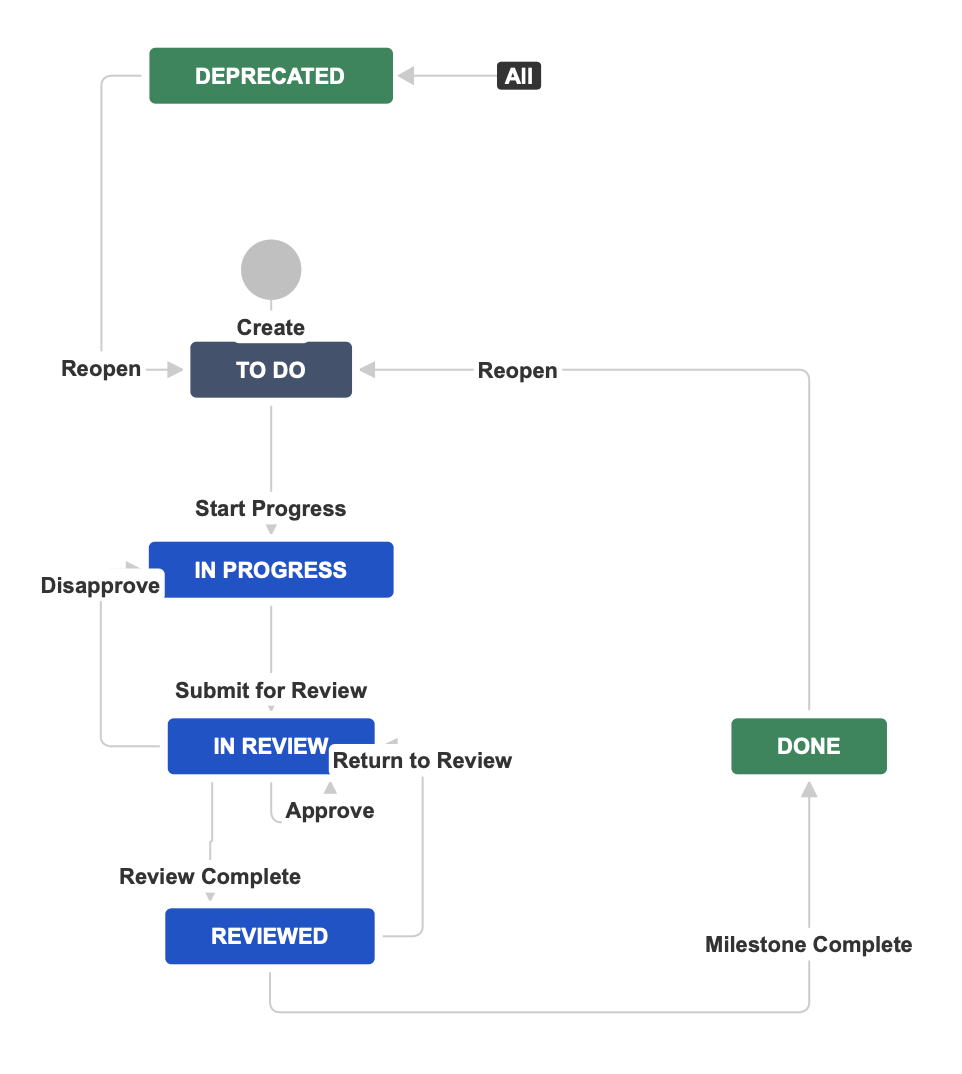
\includegraphics[width=0.48\textwidth]{WorkFlowMilestones.png}
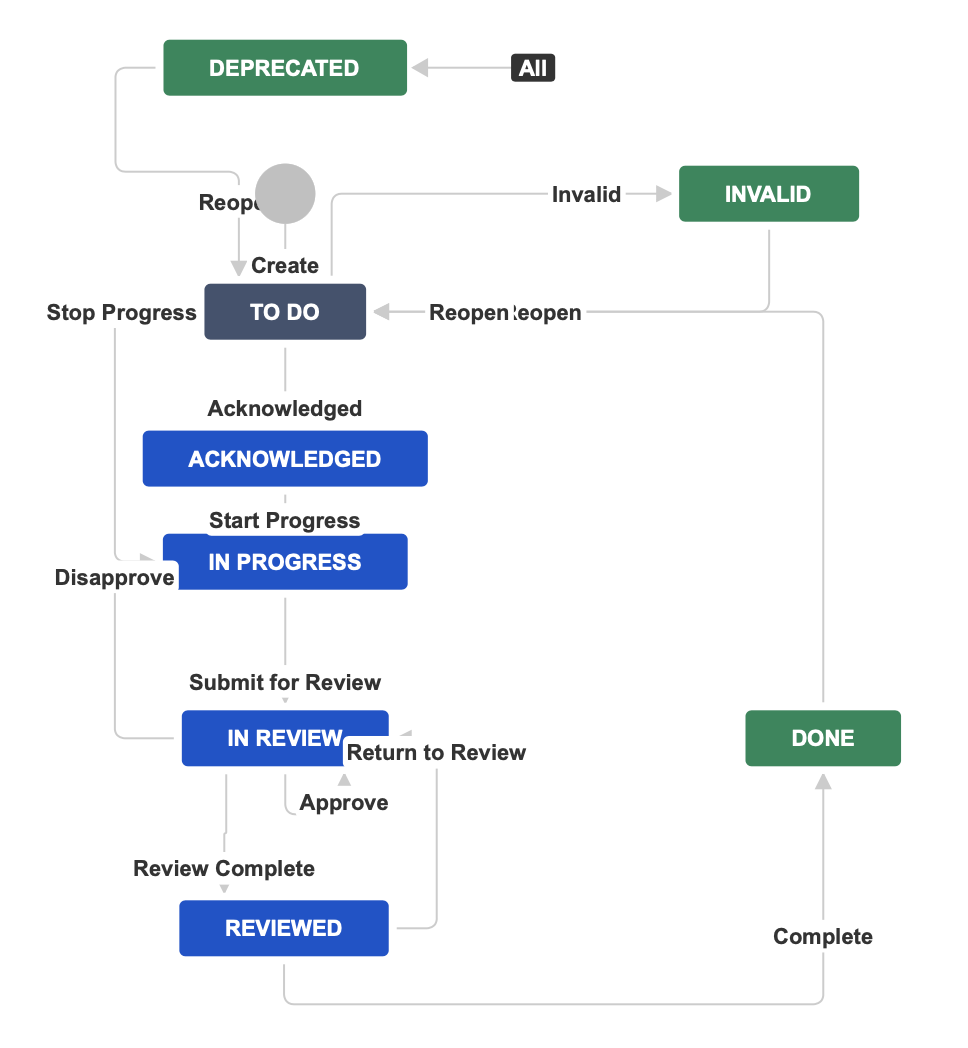
\includegraphics[width=0.48\textwidth]{WorkFlowNonMilestones.png}
\caption{\label{fig:workflow} Workflows}
\end{center}
\end{figure}


\subsection{Ticket Creation and Review process}
To enforce a common process, the workflow has constraints on who is allowed to create tickets and transition them to different state transition. 

Only SIT-COM leads can create, deprecate and/or reopen Milestones tickets. 
SCLT coordinators and leads can create an Epic. 
However, only the assignee can invalidate, deprecate, reopen and/or complete the Epic. 
Stories/bugs are created by a SIT-Com member and the tasks by anyone on the project. 

One particularity of the non-milestone workflow is the required acknowledgement status, only allowed by the assignee, ensuring that the assignee has received the tasks and will act on it. 
As expected, the assignee as well as the start and end dates are required to transition to the acknowledged state.

Regarding the review process, reviewers must be populated before submitting the ticket for Review as an email will automatically be sent to all reviewers as part of the transition. 
All reviewers must approve ticket in order for the ticket to transition to Reviewed status, which is done automatically after the approval from the final reviewer. 
All child and/or included tickets must be approved first. 
In case of disapproval, the system will automatically put the ticket back into In Progress status and only the assignee can send it back to the In Review state. 
Each reviewer is required to add a comment as part of the review process, independently of the outcome. 
The success criteria should be filled in order to guide the reviewers.
The description of the ticket must be sufficiently detailed, including a success criteria when possible, such that the reviewer can properly assess if the task has been completed.
Note that the ticket can not be edited while in the In Review or Reviewed state. 
However, it can be commented on. 


Table \ref{tab:owner} summarizes the ownership of the creation and review process of each SIT-Com Jira ticket. 
\begin{table}
\begin{center}
\caption{\label{tab:owner} Summary of Ownership}
\begin{tabular}{|p{1.8cm}|p{1.8cm}|p{1.8cm}|p{1.8cm}|p{1.8cm}|p{1.8cm}}
\hline
Ticket type vs Use Case              & Milestone 2	& Milestone 3& Epics	& Story/Bug	& Tasks \\
\hline
\hline
Milestone Tracking & {\bf Reporter}: P6 &{\bf Reporter}: P6& {\bf Origin}: One SCLT Coordinator & {\bf Reporter}: SIT-Com member & {\bf Reporter}: Anyone \\
 & {\bf Reviewer}: SIT-Com manager or delegate & {\bf Reviewer}: one SCLT lead or manager & {\bf Reviewer}: one SCLT lead & {\bf Reviewer}: chosen by the ticket reporter or a SCLT coordinator & {\bf Reviewer}: chosen by the ticket reporter or a SCLT coordinator \\
\hline
Planned activities & -- & -- & Same as above & Same as above & Same as above \\
\hline
Emergent issues & -- & -- & -- & Same as above & Same as above \\
\hline
\end{tabular}
\end{center}
\end{table}

\subsection{Linking to Other Jira Projects}
\label{sec:other_jiras}
This project needs to be integrated with the other already existing Jira projects. 
The following list covers the potential required links.

\begin{itemize}
\item Summit: this is the Jira project used to define the activities being conducted at the summit facilities everyday. These activities are ranked by priorities 1 to 4.  The SIT-Com tasks will appear on the summit calendar.
\item DM: the DM project gathered all the activities (planned, bugs, etc) conducted by the software team at large. It includes the pipeline as well as the control software tasks. 
\item IT: the IT project is reserved for all the activities conducted by the IT group, both at the summit, in Tucson and in La Serena. Similarly to the DM project, it covers both planned activities as well as emerging issues. 
\item CAP: CAP stands for the Commissioning Activities Planning and is used for work coordination of software needed for commissioning. There was some discussion to extend this particular Jira project to match our needs, however, there was enough differences that we decided not to go that route. As a result, this project might be merge into the SIT-Com project as we move forward.  
\item LVV: LSST Verification and Validation project gathers all the requirement verification and validation procedures as well as incremental testing procedures.
\item Obs: the Observing Operation Jira project was created for night observation mostly, during which issues are encountered and need to be addressed within the next day or two. Its workflow is basic, allowing for quick reporting, requiring the observer to only add essential details (fault title and description, time of the fault, urgency). The triage and redirection to appropriate assignees and Jira projects is being done by a delegate of each technical group as soon as possible the next day.
\item FRACAS: Failure Reporting, Analysis and Corrective Action System. 
\end{itemize}


\appendix
% Include all the relevant bib files.
% https://lsst-texmf.lsst.io/lsstdoc.html#bibliographies
\section{References} \label{sec:bib}
%\renewcommand{\refname}{} % Suppress default Bibliography section
%\bibliography{local,lsst,lsst-dm,refs_ads,refs,books}
  
% Make sure lsst-texmf/bin/generateAcronyms.py is in your path
\section{Acronyms} \label{sec:acronyms}
\input{acronyms.tex}
% If you want glossary uncomment below -- comment out the two lines above
%\printglossaries





\end{document}
